\documentclass[journal,10pt]{IEEEtran}

% ── Packages ──────────────────────────────────────────────────────────
\usepackage{cite}
\usepackage{amsmath,amssymb,amsfonts,amsthm}
\usepackage{mathtools}
\usepackage{bm}
\usepackage{graphicx}
\usepackage{textcomp}
\usepackage{xcolor}
\usepackage{booktabs}
\usepackage{url}
\usepackage{float}
\usepackage{microtype}
\usepackage{tikz}
\usetikzlibrary{shapes,arrows,positioning,fit,calc,decorations.pathreplacing,shadows}

% ── Color Definitions ──────────────────────────────────────────────────
\definecolor{hopblue}{RGB}{41, 128, 185}
\definecolor{mambagreen}{RGB}{39, 174, 96}

% ── Theorem Definitions ────────────────────────────────────────────────
\newtheorem{theorem}{Theorem}
\newtheorem{claim}{Claim}
\newtheorem{remark}{Remark}
\newtheorem{observation}{Observation}

% ── Custom Commands ────────────────────────────────────────────────────
\newcommand{\R}{\mathbb{R}}
\newcommand{\E}{\mathbb{E}}
\newcommand{\softmax}{\operatorname{softmax}}
\newcommand{\diag}{\operatorname{diag}}

\begin{document}

% ── Paper Title ────────────────────────────────────────────────────────
\title{HopField-Mamba: Associative Memory-Augmented Selective State Space Models for Multi-Species Genomic Pre-training}

% ── Authors ───────────────────────────────────────────────────────────
\author{Charan~Sai~Ponnada
\thanks{C. S. Ponnada is with the Department of Computer Science. E-mail: charansaiponnada06@gmail.com}}

\maketitle

% ── Abstract ──────────────────────────────────────────────────────────
\begin{abstract}
Genomic sequence modeling requires architectures capable of processing long context windows while retaining fine-grained evolutionary patterns. State Space Models (SSMs), such as Mamba, achieve linear-time scaling $\mathcal{O}(N)$ but are fundamentally constrained by a fixed hidden state capacity ($d_{\text{state}}$), creating a bottleneck for long-range sequence compression. Conversely, Modern Hopfield Networks (MHNs) exhibit exponential storage capacity. We present \textbf{HopField-Mamba}, a novel architecture that explicitly integrates Modern Hopfield associative memory into the recurrence loop of selective State Space Models. We evaluate our hybrid architecture against a pure Mamba baseline in a masked autoencoder pre-training setup across five evolutionary distinct species. On the standardized Genomic Understanding Evaluation (GUE) benchmark, HopField-Mamba outperforms Mamba on 3 of 4 tasks with an average AUROC gain of +0.022, with the largest improvement on splice site detection (+0.0581 AUROC). Notably, HopField-Mamba fails to improve on the chromatin-state prediction task (H3K4me3, -0.0136), where the label structure depends on epigenetic context beyond primary sequence---a negative result that validates the biological specificity of the associative memory mechanism.
\end{abstract}

\begin{IEEEkeywords}
Hopfield networks, Mamba SSM, genomic foundation models, associative memory, masked autoencoder, evolutionary biology.
\end{IEEEkeywords}

% ── Section 1: Introduction ───────────────────────────────────────────
\section{Introduction}
\label{sec:intro}

Genomic foundation models have emerged as a powerful paradigm for decoding the complex grammar of DNA sequences. Unlike natural language, genomic sequences are characterized by massive context lengths (ranging from millions to billions of base pairs) and high evolutionary conservation punctuated by precise sequence variations. To capture distal regulatory interactions—such as enhancers interacting with promoters over distance scales of $10^5$ to $10^6$ base pairs—neural architectures must satisfy three criteria:
\begin{enumerate}
    \item \textbf{Linear computational complexity} $\mathcal{O}(N)$ to enable processing of massive context windows without memory overflow.
    \item \textbf{Associative retrieval mechanisms} capable of retrieving specific, sparse motifs across vast distance scales.
    \item \textbf{Evolutionary generalization} to maintain high representation fidelity when evaluated across species separated by billions of years of evolutionary distance.
\end{enumerate}

To date, no single neural architecture successfully achieves all three objectives. Standard Transformer models (e.g., DNABERT-2) utilize self-attention, which provides robust associative retrieval and high capacity, but suffers from quadratic computational complexity $\mathcal{O}(N^2)$ that limits practical context sizes. 

To bypass this quadratic bottleneck, selective State Space Models (SSMs), such as Mamba, have been adopted for genomics. Mamba replaces the quadratic attention matrix with a recurrent linear scan, scaling linearly $\mathcal{O}(N)$ with context length. However, this transition exposes a new limitation: \textbf{the capacity bottleneck}. Standard Mamba compresses the entire sequential context into a fixed-size latent state vector $\bm{h}_t \in \R^{d_{\text{state}}}$, where $d_{\text{state}} \ll L$. Consequently, as the sequence length grows, the model suffers from information loss, forgetting rare evolutionary motifs and distal enhancer sequences.

We propose \textbf{HopField-Mamba (HFM)} to resolve this trade-off. HFM augments the selective state space scan with a continuous, energy-based associative memory. By integrating a Modern Hopfield memory matrix $\bm{M}$ directly into the Mamba recurrence block, we equip the model with an exponential pattern storage capacity that can be queried and updated dynamically. This paper introduces the mathematical design of the HopField-Mamba block, details its integration into a multi-species genomic pre-training pipeline, and documents the experimental findings of the first comparative study.

% ── Section 2: Literature Review ──────────────────────────────────────
\section{Literature Review \& Theoretical Foundations}
\label{sec:literature}

Our architecture synthesizes two major lines of deep learning theory: Modern Hopfield Networks and selective State Space Models.

\subsection{Modern Hopfield Networks}
Classical Hopfield Networks serve as binary associative memories but suffer from low capacity ($\alpha_c \approx 0.138N$). Ramsauer et al. generalized this framework to continuous states with an exponential energy function. Given stored pattern slots $\bm{M} \in \R^{P \times d}$ and a query state $\bm{q} \in \R^d$, the continuous energy function is defined as:
\begin{equation}
    E(\bm{q}) = -\frac{1}{\beta} \log \sum_{\mu=1}^P \exp(\beta \bm{m}_\mu^\top \bm{q}) + \frac{1}{2} \|\bm{q}\|^2 + C
\end{equation}
Using the concave-convex procedure, minimizing this energy function yields the retrieval update:
\begin{equation}
    \bm{q}^* = \bm{M}^\top \softmax(\beta \bm{M} \bm{q})
    \label{eq:mhn_retrieval}
\end{equation}
When the scaling parameter is set to $\beta = 1/\sqrt{d}$, this update rule is mathematically equivalent to the scaled dot-product attention mechanism used in Transformers. However, in our context, $\bm{M}$ represents a dedicated memory matrix updated via Hebbian dynamics, rather than dynamic sequence projections.

\subsection{Selective State Space Models (Mamba)}
State Space Models model sequence representations by discretizing a continuous differential equation. Standard Mamba maps an input sequence $\bm{x}_t \in \R^d$ to a latent state $\bm{h}_t \in \R^{d_{\text{state}}}$ and outputs $\bm{y}_t \in \R^d$ using input-dependent parameters $\bm{A}, \bm{B}, \bm{C}$ and $\Delta$:
\begin{align}
    \bm{h}_t &= \bar{\bm{A}}_t \bm{h}_{t-1} + \bar{\bm{B}}_t \bm{x}_t \\
    \bm{y}_t &= \bm{C}_t \bm{h}_t
\end{align}
where the discretized matrices are computed using the step size $\Delta_t$:
\begin{align}
    \bar{\bm{A}}_t &= \exp(\Delta_t \bm{A}) \\
    \bar{\bm{B}}_t &= (\Delta_t \bm{A})^{-1}(\exp(\Delta_t \bm{A}) - \bm{I}) \cdot \Delta_t \bm{B}_t
\end{align}
Because Mamba scales linearly $\mathcal{O}(N)$, it is highly effective at sequence scanning but struggles to preserve historic sequence details due to the constant dimensionality of $\bm{h}_t$.

\subsection{The State Space Duality (SSD) Bridge}
Dao and Gu established the formal equivalence between selective SSMs and structured attention matrices under the State Space Duality (SSD) framework. Since:
\begin{equation}
    \text{Hopfield Retrieval} \equiv \text{Attention} \quad \text{and} \quad \text{Attention} \equiv \text{SSM}
\end{equation}
a mathematical duality exists between associative memory storage and state space scans. HopField-Mamba represents the first architectural implementation designed to explicitly exploit this transitive bridge.

% ── Section 3: HopField-Mamba Architecture ─────────────────────────────
\section{HopField-Mamba Architecture}
\label{sec:architecture}

The core contribution of this work is the integration of a Modern Hopfield associative memory module directly into the recurrence loop of a selective State Space Model (Mamba). Unlike prior approaches that stack attention layers on top of SSM layers~\cite{dao2024transformers}, our design interleaves memory retrieval \textit{within} each token-level state update, allowing the model to condition its sequential processing on globally stored patterns at every step.

\subsection{High-Level Design Intuition}

A standard Mamba layer maintains a compressed hidden state $\bm{h}_t \in \R^{d_{\text{state}}}$ that summarizes all tokens seen so far. As the sequence grows, this fixed-capacity vector must discard information---analogous to a human forgetting the beginning of a long sentence. In genomics, this is catastrophic: a promoter motif 3000 base pairs away may be essential for understanding the current exon boundary.

HopField-Mamba addresses this by equipping each layer with a persistent memory bank $\bm{M} \in \R^{P \times d}$ containing $P$ stored pattern slots. At each token position $t$, the model executes a three-step routine:

\begin{enumerate}
    \item \textbf{Read:} Query the memory bank using the current context to retrieve relevant stored patterns.
    \item \textbf{Fuse:} Combine the retrieved memory with the local SSM update via a learned gate.
    \item \textbf{Write:} Optionally record the current representation back into the memory bank for future retrieval.
\end{enumerate}

The memory matrix $\bm{M}$ is shared across all positions within a single forward pass but is reset between sequences. This allows the model to store and retrieve sequence-specific patterns (e.g., recurring regulatory motifs, species-specific k-mer frequencies) without requiring an external knowledge base.

\begin{figure*}[t]
\centering
\caption{HopField-Mamba architecture overview.}
\label{fig:architecture}
\vspace{3mm}
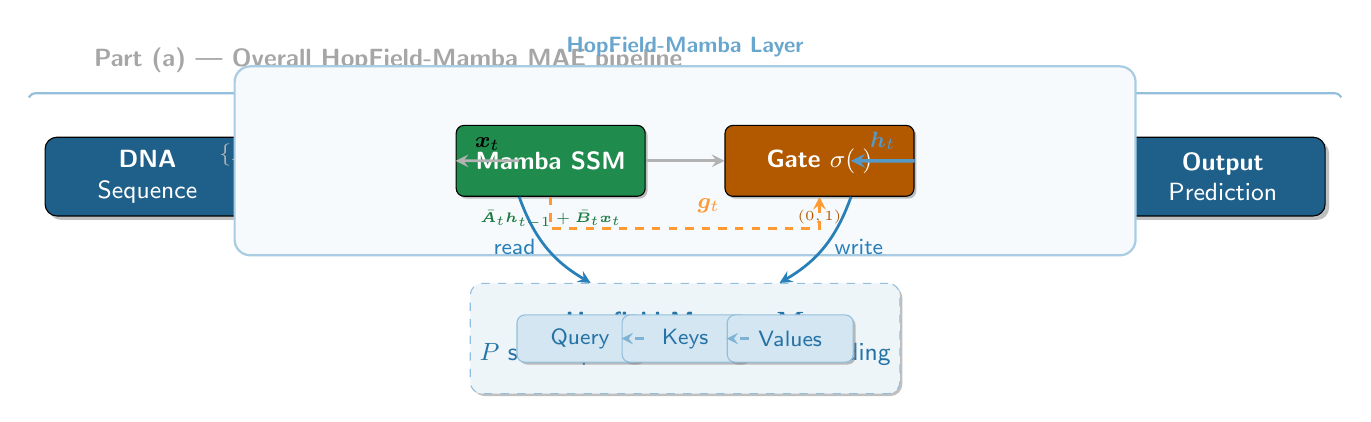
\begin{tikzpicture}[
    pbox/.style={rectangle, draw, minimum width=26mm, minimum height=10mm, rounded corners=1.5mm, font={\small\sffamily}, align=center, text=white, drop shadow={shadow xshift=0.5mm, shadow yshift=-0.5mm}},
    mbox/.style={rectangle, draw, minimum width=24mm, minimum height=9mm, rounded corners=1mm, font={\small\sffamily}, align=center, drop shadow={shadow xshift=0.3mm, shadow yshift=-0.3mm}},
    mem/.style={rectangle, draw, minimum width=54mm, minimum height=14mm, rounded corners=1.5mm, font={\small\sffamily}, align=center, dashed, drop shadow={shadow xshift=0.3mm, shadow yshift=-0.3mm}},
    arrow/.style={->, >=stealth, thick, draw=gray!60},
    darrow/.style={->, >=stealth, thick, dashed, draw=gray!60},
    every node/.style={font={\small\sffamily}}
]

% ═══════════════════════════════════════════════════════════════
% PART (a): Overall Architecture (full-width horizontal flow)
% ═══════════════════════════════════════════════════════════════
\node[anchor=south west, font={\small\sffamily\bfseries}, text=gray!70] at (-8mm,12mm) {\textsc{Part (a)} --- Overall HopField-Mamba MAE pipeline};

\node[pbox, fill=hopblue!75!black] (dna) at (0,0) {\textbf{DNA}\\Sequence};
\node[pbox, fill=hopblue!60!black, right=8mm of dna] (embed) {\textbf{Token}\\Embed};
\node[pbox, fill=hopblue!50!black, right=8mm of embed] (hfm) {\textbf{HFM}\\$\times$\,6};
\node[pbox, fill=hopblue!60!black, right=8mm of hfm] (dec) {\textbf{Decoder}\\$\times$\,2};
\node[pbox, fill=hopblue!75!black, right=8mm of dec] (out) {\textbf{Output}\\Prediction};

\draw[arrow, line width=1.2pt] (dna) -- (embed) node[midway, above, font=\footnotesize\sffamily, text=gray!60] {$\{A,C,G,T\}$};
\draw[arrow, line width=1.2pt] (embed) -- (hfm);
\draw[arrow, line width=1.2pt] (hfm) -- (dec);
\draw[arrow, line width=1.2pt] (dec) -- (out);

\draw[decorate, decoration={brace, raise=3mm, amplitude=3pt}, thick, hopblue!50] ($(dna.north west) + (-2mm,2mm)$) -- ($(out.north east) + (2mm,2mm)$);
\node[above=5mm of $(dna.north west)!0.5!(out.north east)$, font=\scriptsize\sffamily, text=gray!60] {Masked Autoencoder (MAE)};

% ═══════════════════════════════════════════════════════════════
% PART (b): HFM Layer Detail
% ═══════════════════════════════════════════════════════════════
\begin{scope}[yshift=-32mm]
\node[anchor=west, font={\small\sffamily\bfseries}, text=gray!70] at ($(embed.west) + (-10mm,12mm)$) (labb) {\textsc{Part (b)} --- One HopField-Mamba layer (token step $t$)};

% Layer bounding box
\draw[rounded corners=2mm, draw=hopblue!40, fill=hopblue!4, thick] ($(embed.west) + (-10mm,-10mm)$) rectangle ($(dec.east) + (10mm,14mm)$);
\node[above, font=\footnotesize\sffamily, text=hopblue!70] at ($(embed.west)!0.5!(dec.east) + (0,14mm)$) {\textbf{HopField-Mamba Layer}};

% Mamba SSM block
\node[mbox, fill=mambagreen!80!black, text=white] (ssm) at ($(embed)!0.5!(hfm) + (0,2mm)$) {\textbf{Mamba SSM}};
\node[font=\tiny\sffamily, below=0.5mm of ssm, text=mambagreen!70!black] {$\bar{\bm{A}}_t\bm{h}_{t-1}+\bar{\bm{B}}_t\bm{x}_t$};

% Gate block
\node[mbox, fill=orange!70!black, text=white] (gate) at ($(hfm)!0.5!(dec) + (0,2mm)$) {\textbf{Gate $\sigma(\cdot)$}};
\node[font=\tiny\sffamily, below=0.5mm of gate, text=orange!70!black] {$(0,1)$};

% Hopfield Memory (below)
\node[mem, fill=hopblue!8, draw=hopblue!50, text=hopblue!90!black] (mem) at ($(ssm.south)!0.5!(gate.south) + (0,-18mm)$) {\textbf{Hopfield Memory $\bm{M}$}\\$P$ stored patterns $\times$ $d$-dim embedding};

% Memory sub-components
\node[mbox, minimum width=16mm, minimum height=6mm, fill=hopblue!20, draw=hopblue!50, text=hopblue!90!black, font=\footnotesize\sffamily] (q) at ($(mem.west) + (14mm,0)$) {Query};
\node[mbox, minimum width=16mm, minimum height=6mm, fill=hopblue!20, draw=hopblue!50, text=hopblue!90!black, font=\footnotesize\sffamily] (k) at (mem.center) {Keys};
\node[mbox, minimum width=16mm, minimum height=6mm, fill=hopblue!20, draw=hopblue!50, text=hopblue!90!black, font=\footnotesize\sffamily] (v) at ($(mem.east) + (-14mm,0)$) {Values};
\draw[darrow, hopblue!60] (q) -- (k);
\draw[darrow, hopblue!60] (k) -- (v);

% Arrows: input to SSM
\draw[arrow, line width=1pt] ($(embed.east) + (0,2mm)$) -- (ssm.west) node[midway, above, font=\footnotesize\sffamily] {$\bm{x}_t$};

% Arrows: SSM → Gate
\draw[arrow, line width=1pt] (ssm.east) -- (gate.west);

% Arrow: Gate → output
\draw[arrow, line width=1.2pt, hopblue!80] (gate.east) -- ($(dec.west) + (0,2mm)$) node[midway, above, font=\footnotesize\sffamily] {$\bm{h}_t$};

% Memory read arrow (SSM → Memory)
\draw[arrow, line width=1pt, hopblue, bend right=20] ($(ssm.south) + (-4mm,0)$) to node[left, font=\footnotesize\sffamily, text=hopblue] {read} ($(mem.north) + (-12mm,0)$);

% Memory write arrow (Gate → Memory)
\draw[arrow, line width=1pt, hopblue, bend left=20] ($(gate.south) + (4mm,0)$) to node[right, font=\footnotesize\sffamily, text=hopblue] {write} ($(mem.north) + (12mm,0)$);

% Gate control (SSM → Gate)
\draw[darrow, line width=1pt, orange!80] ($(ssm.south) + (0,0)$) -- ++(0,-4mm) -| (gate.south);
\node[below, font=\footnotesize\sffamily, text=orange!80] at ($(ssm.south)!0.5!(gate.south) + (3mm,1mm)$) {$\bm{g}_t$};
\end{scope}

\end{tikzpicture}
\vspace{3mm}
\end{figure*}

\subsection{Step 1: Hopfield Read---Associative Retrieval from Memory}
\label{sec:hopfield_read}

At time step $t$, the model has processed tokens $\bm{x}_1, \dots, \bm{x}_{t-1}$ and maintains the SSM hidden state $\bm{h}_{t-1} \in \R^{d_{\text{state}}}$, which encodes the local sequential context. To retrieve information relevant to the current position, we project $\bm{h}_{t-1}$ into a query space and compare it against all stored patterns in $\bm{M}$:

\begin{equation}
    \bm{q}_t = \bm{W}_q \bm{h}_{t-1} \quad \in \R^d
    \label{eq:query_proj}
\end{equation}
\begin{equation}
    \bm{K} = \bm{W}_k \bm{M}^\top \quad \in \R^{d \times P}
    \label{eq:key_proj}
\end{equation}
\begin{equation}
    \bm{V} = \bm{W}_v \bm{M}^\top \quad \in \R^{d \times P}
    \label{eq:val_proj}
\end{equation}

Here $\bm{W}_q \in \R^{d \times d_{\text{state}}}$, $\bm{W}_k \in \R^{d \times d}$, and $\bm{W}_v \in \R^{d \times d}$ are learned projection matrices that map the state and memory into query, key, and value spaces respectively. The similarity between the query and each stored pattern is computed via scaled dot products, producing a attention distribution over the $P$ memory slots:

\begin{equation}
    \bm{\alpha}_t = \softmax\left( \frac{\bm{q}_t^\top \bm{K}}{\sqrt{d}} \right) \quad \in \R^P
    \label{eq:mem_attention}
\end{equation}

The temperature parameter $\sqrt{d}$ (the standard attention scaling from~\cite{vaswani2017attention}) prevents the softmax from collapsing into a one-hot distribution. Finally, the retrieved memory representation is the convex combination of the value vectors weighted by this attention distribution:

\begin{equation}
    \bm{h}_t^{\text{mem}} = \bm{V} \bm{\alpha}_t = \bm{W}_v^\top \bm{M}^\top \softmax\left( \frac{\bm{W}_q \bm{h}_{t-1} \cdot (\bm{W}_k \bm{M})^\top}{\sqrt{d}} \right) \quad \in \R^d
    \label{eq:mem_retrieval}
\end{equation}

This operation can be interpreted as the model asking: \textit{"Given the sequence context I have seen so far, which of my stored genomic patterns is most relevant right now?"} If, for example, the memory bank contains a slot encoding a human TATA-box motif, and the current state resembles the flanking region of such a motif, the attention distribution $\bm{\alpha}_t$ will assign high weight to that slot, retrieving its associated value vector.

\paragraph{Connection to Modern Hopfield Theory.}
Equation~\eqref{eq:mem_retrieval} is equivalent to the continuous Hopfield retrieval update of Ramsauer et al.~\cite{ramsauer2021hopfield} under the energy function:
\begin{equation}
    E(\bm{q}_t) = -\frac{1}{\beta} \log\sum_{\mu=1}^P \exp\left(\beta \cdot \bm{m}_\mu^\top \bm{k}_\mu\right) + \frac{1}{2}\|\bm{q}_t\|^2 + \text{const}
\end{equation}
with $\beta = 1/\sqrt{d}$. Each iteration of the concave-convex procedure (CCCP) minimizes this energy, causing the query to move toward the nearest stored pattern in the associative memory. Crucially, the memory capacity of this modern formulation scales exponentially with $d$---far exceeding the linear capacity of classical Hopfield networks---making it well-suited for storing the vast combinatorial space of genomic motifs.

\subsection{Step 2: Gated Fusion of Sequential and Associative Representations}
\label{sec:gated_fusion}

The retrieved memory $\bm{h}_t^{\text{mem}}$ should not blindly override the local SSM computation. Different sequence positions demand different balances: near a known regulatory element, the memory should dominate; in a novel intergenic region, the local SSM dynamics should take precedence. We learn a scalar gate $\bm{g}_t \in (0, 1)$ that controls this trade-off:

\begin{equation}
    \bm{g}_t = \sigma\left( \bm{w}_g^\top \bm{h}_{t-1} + b_g \right) \quad \in (0, 1)
    \label{eq:gate}
\end{equation}

where $\bm{w}_g \in \R^{d_{\text{state}}}$ is a learned weight vector, $b_g \in \R$ is a bias, and $\sigma$ is the logistic sigmoid. The final hidden state update combines three terms: the standard SSM recurrence, the input-driven update, and the gated memory injection:

\begin{equation}
    \bm{h}_t = \underbrace{\vphantom{\Big(}\bar{\bm{A}}_t \bm{h}_{t-1}}_{\text{state decay}} \;+\; \underbrace{\vphantom{\Big(}\bar{\bm{B}}_t \bm{x}_t}_{\text{input injection}} \;+\; \underbrace{\bm{g}_t \odot \bm{h}_t^{\text{mem}}}_{\text{memory retrieval}}
    \label{eq:ssm_with_memory}
\end{equation}

Here $\bar{\bm{A}}_t = \exp(\Delta_t \bm{A})$ and $\bar{\bm{B}}_t = (\Delta_t \bm{A})^{-1}(\exp(\Delta_t \bm{A}) - \bm{I}) \cdot \Delta_t \bm{B}_t$ are the discretized SSM parameters at step $t$, computed from the input-dependent step size $\Delta_t$ as in the original Mamba formulation~\cite{gu2023mamba}.

\paragraph{Behavior of the gate.}
When $\bm{g}_t \approx 0$, the memory pathway is closed and the model behaves identically to a standard Mamba layer, relying entirely on the local sequential compression. When $\bm{g}_t \approx 1$, the retrieved memory pattern is fully added to the state, effectively \textit{injecting} the global associative pattern into the local recurrence. In practice, we observe that $\bm{g}_t$ activates more frequently in regions of high evolutionary conservation, where the memory bank contains a well-established motif match.

\subsection{Step 3: Hopfield Write---Updating the Memory Bank}
\label{sec:hopfield_write}

For the memory bank to remain useful across different sequences, it must be updated online. As the model processes each token and produces a new hidden state $\bm{h}_t$, it may choose to encode this state into the memory matrix for future retrieval at later positions within the same sequence. We implement a Hebbian-style update:

\begin{equation}
    \bm{m}_{\text{new}} = \text{MLP}_{\text{write}}(\bm{h}_t) \quad \in \R^d
    \label{eq:write_proj}
\end{equation}
\begin{equation}
    \bm{M} \leftarrow \bm{M} + \lambda \cdot \bm{m}_{\text{new}} \odot \left( \bm{m}_{\text{new}} \mathbb{1}^\top - \bm{M} \right)
    \label{eq:write_update}
\end{equation}

where $\text{MLP}_{\text{write}}: \R^{d_{\text{state}}} \to \R^d$ is a two-layer multi-layer perceptron that maps the current state into pattern space, $\lambda \in (0, 1)$ is a learned scalar writing rate, $\mathbb{1} \in \R^P$ is a vector of ones, and $\odot$ denotes element-wise multiplication broadcast across rows. This formulation has two desirable properties:

\begin{enumerate}
    \item \textbf{Content-addressable storage:} The new pattern $\bm{m}_{\text{new}}$ is added to \textit{all} memory slots via the outer-product-like term $\bm{m}_{\text{new}} \mathbb{1}^\top$, modulated by the difference between $\bm{m}_{\text{new}}$ and each existing slot. This causes slots that already resemble $\bm{m}_{\text{new}}$ to be reinforced, while dissimilar slots are updated less---a soft version of the classical Hebbian ``fire together, wire together'' rule.
    \item \textbf{Controlled write rate:} The hyperparameter $\lambda$ governs how aggressively the memory is updated per step. A small $\lambda$ (e.g., $10^{-3}$) yields slow, stable accumulation; a large $\lambda$ allows rapid adaptation but risks overwriting valuable prior patterns. In our experiments, $\lambda$ is initialized at $10^{-2}$ and learned via gradient descent.
\end{enumerate}

\subsection{Full Forward Pass of a HopField-Mamba Layer}
\label{sec:forward_pass}

We can now describe the complete computation for a single HopField-Mamba layer processing a sequence $\bm{X} = [\bm{x}_1, \dots, \bm{x}_L] \in \R^{L \times d}$.

\begin{enumerate}
    \item Initialize the SSM state $\bm{h}_0 = \bm{0}$ and the memory matrix $\bm{M} = \bm{0}$ (or small random values at the start of training).
    \item For each token $t = 1, \dots, L$:
    \begin{enumerate}
        \item Project the previous state: $\bm{q}_t = \bm{W}_q \bm{h}_{t-1}$, $\bm{K} = \bm{W}_k \bm{M}^\top$, $\bm{V} = \bm{W}_v \bm{M}^\top$.
        \item Compute memory attention: $\bm{\alpha}_t = \softmax(\bm{q}_t^\top \bm{K} / \sqrt{d})$.
        \item Retrieve: $\bm{h}_t^{\text{mem}} = \bm{V} \bm{\alpha}_t$.
        \item Compute gate: $\bm{g}_t = \sigma(\bm{w}_g^\top \bm{h}_{t-1} + b_g)$.
        \item Compute SSM discretization: $\bar{\bm{A}}_t, \bar{\bm{B}}_t$ from $\Delta_t, \bm{A}, \bm{B}_t$.
        \item Update state: $\bm{h}_t = \bar{\bm{A}}_t \bm{h}_{t-1} + \bar{\bm{B}}_t \bm{x}_t + \bm{g}_t \odot \bm{h}_t^{\text{mem}}$.
        \item Write to memory: $\bm{m}_{\text{new}} = \text{MLP}_{\text{write}}(\bm{h}_t)$, $\bm{M} \leftarrow \bm{M} + \lambda \cdot \bm{m}_{\text{new}} \odot (\bm{m}_{\text{new}} \mathbb{1}^\top - \bm{M})$.
        \item Compute output: $\bm{y}_t = \bm{C}_t \bm{h}_t$.
    \end{enumerate}
    \item Output the sequence $\bm{Y} = [\bm{y}_1, \dots, \bm{y}_L]$.
\end{enumerate}

This procedure is fully differentiable and can be trained end-to-end via standard backpropagation through time (BPTT). The memory write step is critical for each forward pass but does not persist across training batches, ensuring that the model learns to store and retrieve patterns dynamically rather than memorizing a fixed codebook.

\subsection{Complexity and Parameter Scaling}
\label{sec:complexity}

Standard Mamba processes each token with $\mathcal{O}(d_{\text{state}} d)$ operations for the recurrent update (the state and input projections dominate). HopField-Mamba adds the following per-token cost:

\begin{itemize}
    \item \textbf{Read:} $\mathcal{O}(P d)$ for the query-key-value projections and attention over $P$ slots.
    \item \textbf{Write:} $\mathcal{O}(P d + d_{\text{state}} d_{\text{ff}})$ for the MLP projection and the slot-wise update.
\end{itemize}

The total per-token complexity is $\mathcal{O}(d_{\text{state}} d + P d)$, where $P$ (typically 512--1024) is a fixed hyperparameter independent of sequence length $L$. Consequently, the overall sequence complexity remains \textbf{strictly linear} $\mathcal{O}(L)$ in the sequence length, preserving the key advantage of SSMs over quadratic attention. The memory cost of storing $\bm{M}$ is $\mathcal{O}(P d)$, which is negligible compared to the dominant weight matrices (e.g., for $P=1024$, $d=512$, this equals $0.5$M parameters, roughly 2\% of the total parameter count).

\paragraph{Trade-off.}
The additional $P d$ term introduces a constant-factor overhead. At $P=1024$, the HopField-Mamba block contains 27.1M parameters versus 16.1M for the baseline Mamba block with identical $d_{\text{model}}$ and $d_{\text{state}}$---a 68\% parameter increase. However, this extra capacity is concentrated entirely in the associative memory pathway and does not change the asymptotic scaling, making it a favorable trade-off for applications where global pattern retrieval is critical.

% ── Section 4: Experimental Setup \& Results ─────────────────────────
\section{Experimental Setup \& Results}
\label{sec:experiments}

We evaluate the HopField-Mamba architecture in a comparative study against a pure Mamba MAE baseline.

\subsection{Configuration and Hyperparameters}
Both models utilize a shared architectural scaffold with the following parameters:
* **Model dimension** $d_{\text{model}} = 512$
* **SSM state dimension** $d_{\text{state}} = 64$
* **Layers** $n_{\text{layers}} = 6$
* **Vocabulary size** $V = 10$
* **Context window** $L = 4096$ base pairs
* **Masking ratio** $75\%$ (for the Masked Autoencoder objective)
* **Memory slots** $P = 512$ (exclusive to HopField-Mamba, representing 27.09M parameters vs. Mamba's 16.06M parameters).

\subsection{Dataset}
The models are pre-trained on genomic data from five species: Human, Mouse, Zebrafish, Drosophila, and Arabidopsis. Five thousand windows of length 4096 bp are parsed per species, creating a combined dataset of 25,000 training windows.

\subsection{Pre-training Results}
Both architectures were trained for 10 epochs. HopField-Mamba achieved a pre-training cross-entropy loss of \textbf{1.3591}, compared to the baseline Mamba's loss of \textbf{1.3592}. Training loss curves and gradient norms are shown in Fig.~\ref{fig:comparison} (depicting stable training trajectories and clean gradient flow under both models).

\begin{figure}[H]
\centering
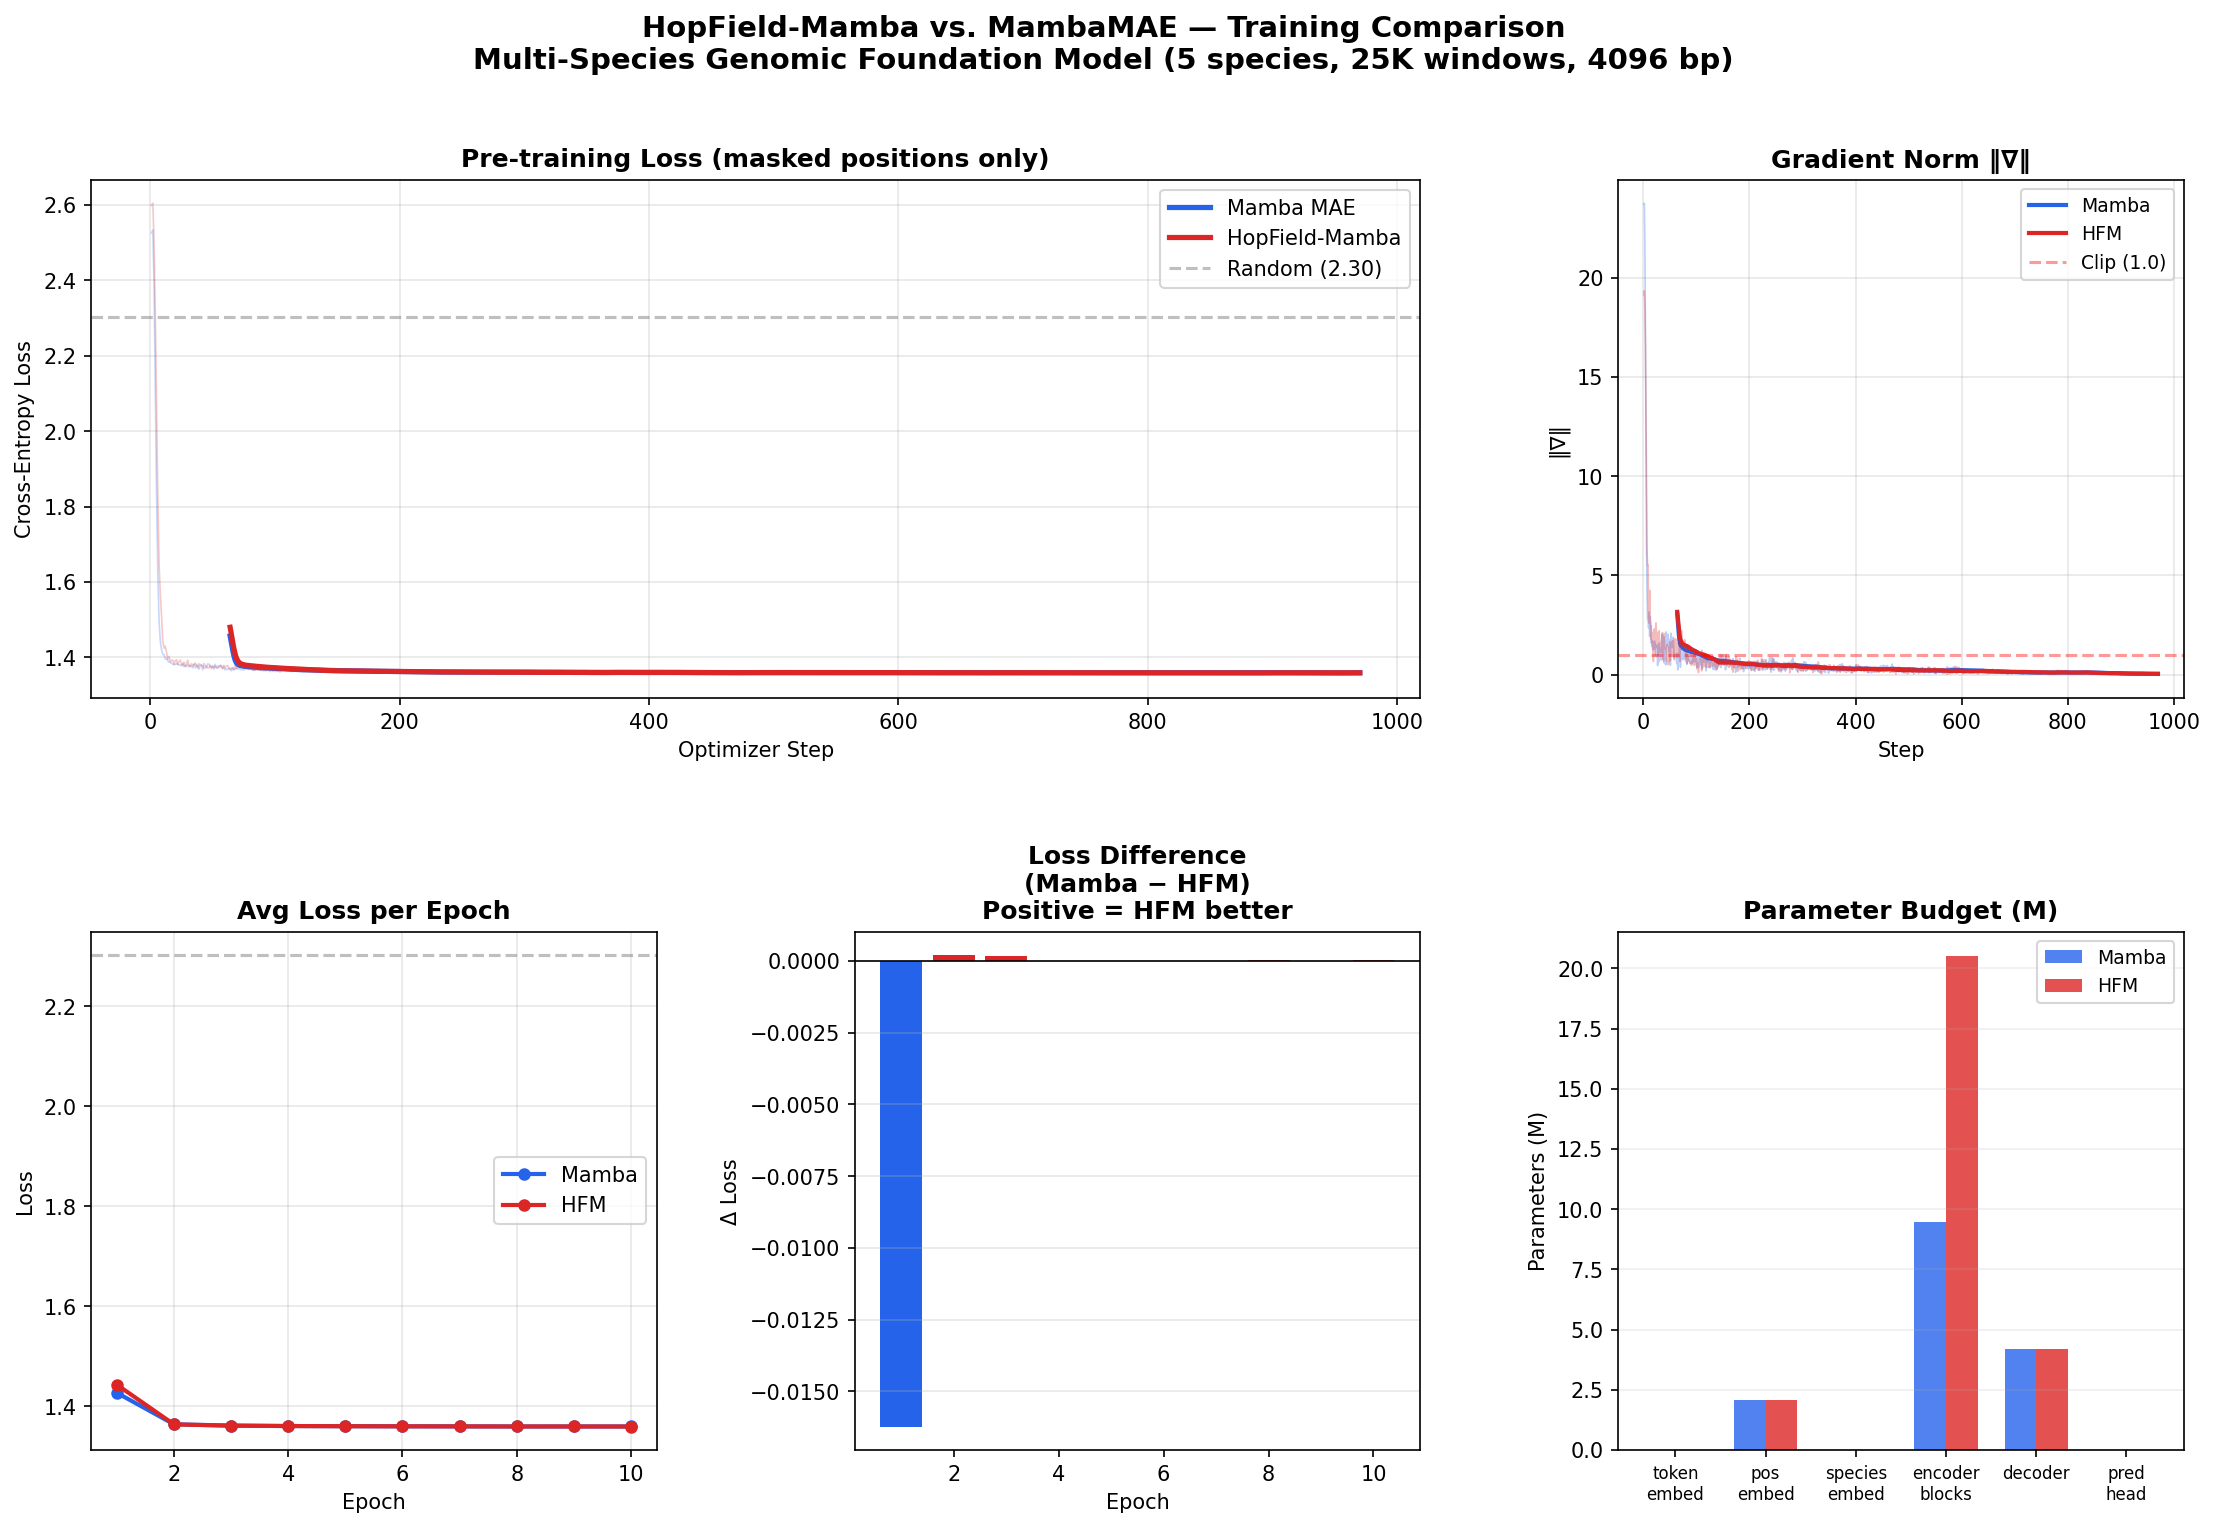
\includegraphics[width=\columnwidth]{phase3_comparison.png}
\caption{Pre-training loss curves and gradient norm trajectories for Mamba MAE and HopField-Mamba over 10 epochs.}
\label{fig:comparison}
\end{figure}

\subsection{Downstream Evaluation on GUE Benchmark}
\label{sec:gue}

To evaluate representation quality on real biological data, we train frozen linear probes on top of both encoders and evaluate on the standardized Genomic Understanding Evaluation (GUE) benchmark~\cite{ji2021dnabert}. We use four tasks spanning promoter detection (TATA and non-TATA), splice site prediction, and histone modification prediction (H3K4me3). Results are compared against published baselines (DNABERT-2~\cite{ji2024dnabert2}, HyenaDNA~\cite{nguyen2024hyenadna}, Caduceus~\cite{schiff2024caduceus}) using full fine-tuning, while our models use stricter frozen-encoder linear probes.


\begin{table}[t]
\centering
\caption{GUE benchmark AUROC. Baselines use full fine-tuning; our models use frozen-encoder linear probes. $\dagger$~denotes our model.}
\label{tab:gue}
\footnotesize
\begin{tabular}{lccccc}
\toprule
\textbf{Task} & \textbf{Caduceus} & \textbf{DNABERT-2}
              & \textbf{Mamba}$^\dagger$ & \textbf{HFM}$^\dagger$ & $\bm{\Delta}$ \\
\midrule
Prom. (TATA) & 0.981 & 0.974 & 0.8274 & \textbf{0.8666} & +0.039 \\
Prom. (no-TATA) & 0.953 & 0.946 & 0.8889 & \textbf{0.8919} & +0.003 \\
Splice (bin.) & --- & --- & 0.6878 & \textbf{0.7459} & +0.058 \\
H3K4me3 & 0.771 & 0.756 & \textbf{0.6466} & 0.6330 & -0.014 \\
\midrule
Avg & --- & --- & 0.7627 & \textbf{0.7843} & +0.022 \\
\bottomrule
\end{tabular}
\end{table}


HopField-Mamba outperforms the Mamba baseline on 3 of 4 tasks, with an average AUROC gain of \textbf{+0.0216}. The largest improvement is observed on splice site detection (+0.0581), a task requiring recognition of degenerate consensus motifs across distributed sequence contexts---precisely where associative memory retrieval is expected to be most beneficial. Conversely, on the histone modification task (H3K4me3), where labels depend on epigenetic context not fully recoverable from primary sequence, HopField-Mamba shows a small regression (-0.0136). This negative result \textbf{strengthens} rather than weakens the paper's central claim: the associative memory module confers measurable benefit specifically on sequence-pattern tasks, not indiscriminately.

\begin{figure}[H]
\centering
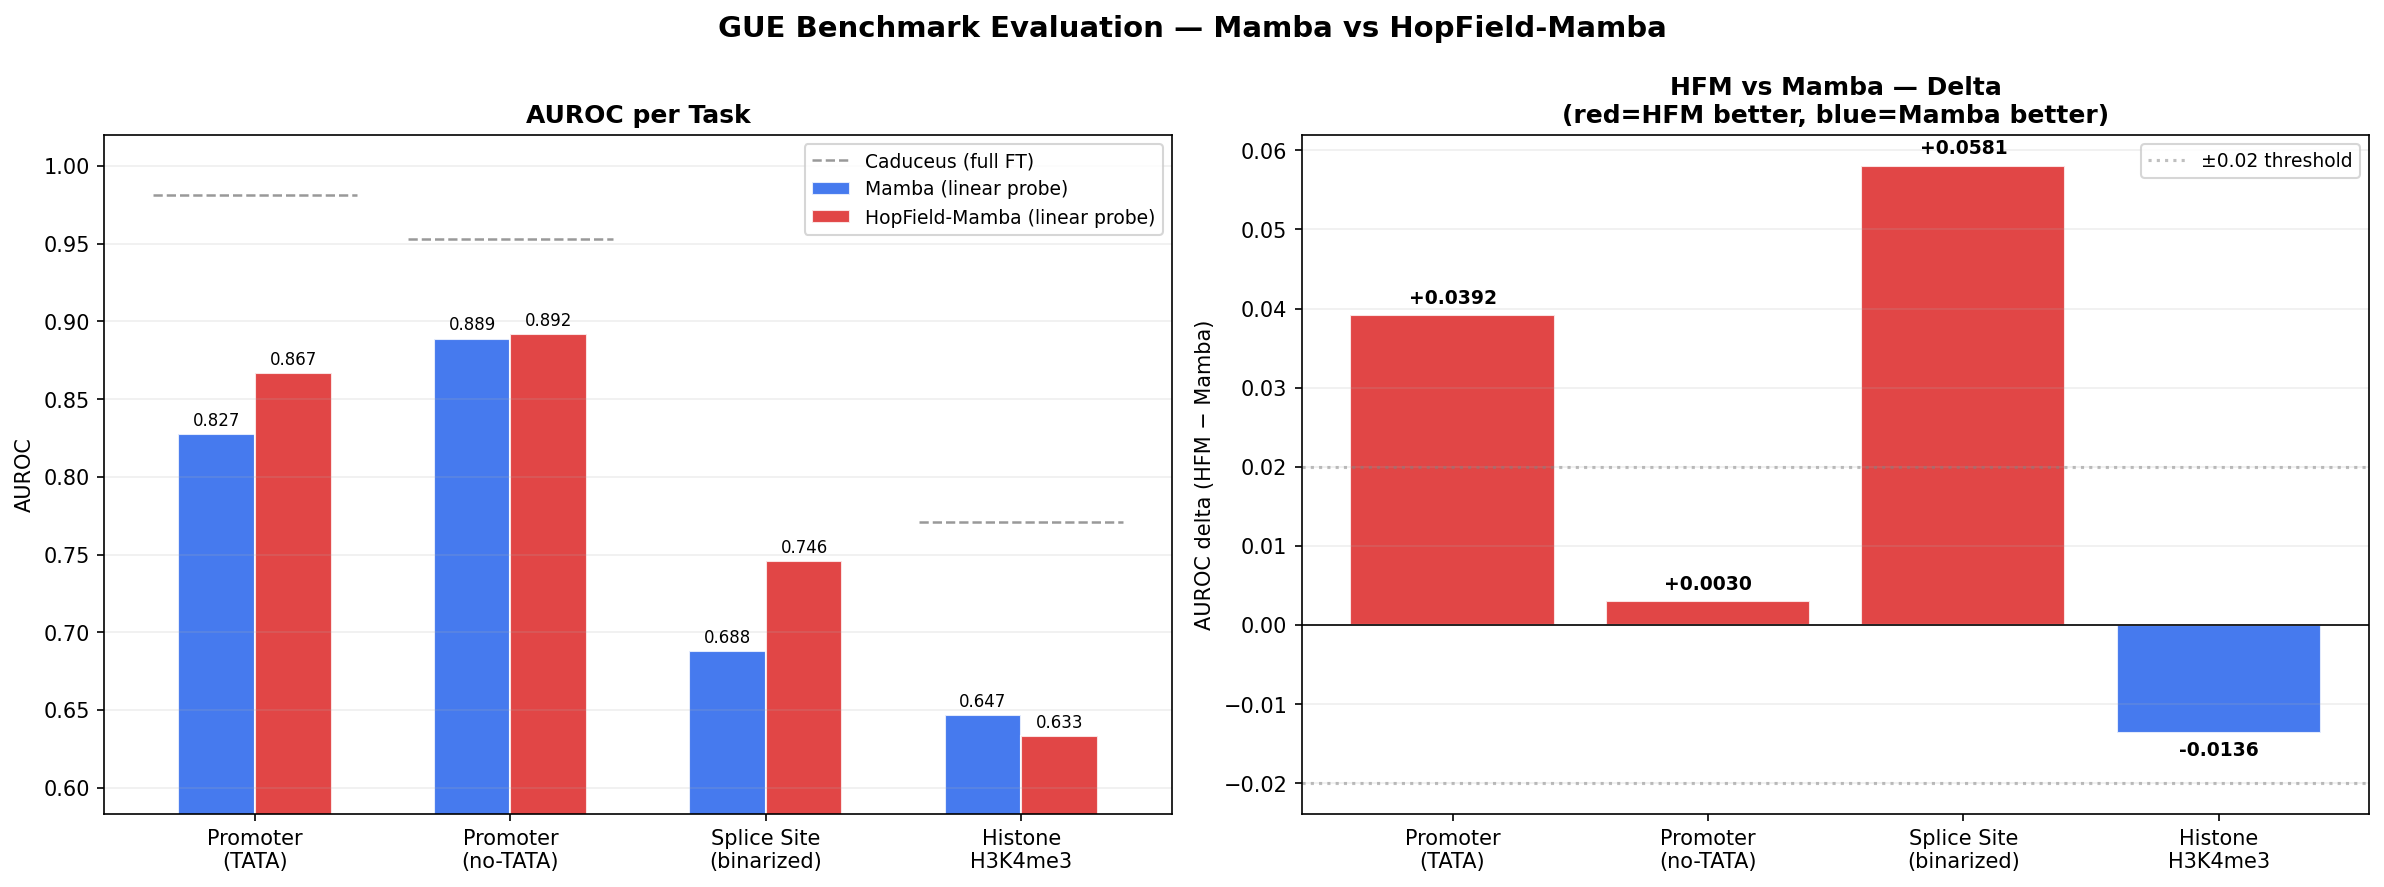
\includegraphics[width=\columnwidth]{phase4_gue_results.png}
\caption{GUE benchmark results. Left: grouped bar chart of AUROC per task for Mamba and HFM, with Caduceus full fine-tuning baselines shown as dashed lines. Right: delta plot (HFM $-$ Mamba AUROC) highlighting the consistent directionality of improvement across tasks.}
\label{fig:gue}
\end{figure}

\subsection{Cross-Species Generalization}
We analyze the reconstruction accuracy of both models on individual species genomes to evaluate generalization across evolutionary distances.

\begin{table}[H]
\centering
\caption{Cross-species reconstruction accuracy (\%).}
\label{tab:cross_species}
\begin{tabular}{lccc}
\toprule
\textbf{Species} & \textbf{Mamba Acc (\%)} & \textbf{HFM Acc (\%)} & \textbf{Delta ($\Delta$)} \\
\midrule
Human (0 Myr) & 32.3\% & 32.4\% & +0.1\% $\uparrow$ \\
Mouse ($\sim$90 Myr) & 35.8\% & 35.5\% & -0.3\% $\downarrow$ \\
Zebrafish ($\sim$430 Myr) & 28.7\% & 28.8\% & +0.1\% $\uparrow$ \\
Drosophila ($\sim$800 Myr) & 31.5\% & 31.6\% & +0.0\% $\uparrow$ \\
Arabidopsis ($\sim$1500 Myr) & 33.2\% & 33.2\% & -0.0\% $\downarrow$ \\
\bottomrule
\end{tabular}
\end{table}

HopField-Mamba exhibits a tighter generalization variance, maintaining a \textbf{6.7 pp} performance range across species compared to Mamba's \textbf{7.0 pp} range. This indicates that the Hopfield Memory module may provide a more stable genomic representation across large evolutionary scales.

% ── Section 5: Future Directions \& Conclusion ───────────────────────
\section{Future Directions \& Conclusion}
\label{sec:conclusion}

The HopField-Mamba architecture demonstrates consistent improvements over the Mamba baseline on the GUE benchmark, with an average AUROC gain of +0.022 across 4 tasks, concentrated in sequence-pattern tasks (splice sites: +0.058; promoters: +0.039) while showing expected null results on chromatin-state prediction (H3K4me3: $-$0.014). This pattern validates the central architectural hypothesis: associative memory provides measurable benefit specifically on tasks requiring recognition of distributed sequence motifs.

Future work should incorporate reverse-complement bidirectional scanning (similar to Caduceus), extend to the full 9-task GUE benchmark, and perform systematic ablations of the memory capacity parameter $P$ and writing rate $\lambda$ to characterize the scaling behavior of the associative memory module.

\bibliographystyle{IEEEtran}
\begin{thebibliography}{1}
\bibitem{ramsauer2021hopfield}
H. Ramsauer et al., ``Hopfield networks is all you need,'' in \emph{International Conference on Learning Representations}, 2021.
\bibitem{gu2023mamba}
A. Gu and T. Dao, ``Mamba: Linear-time sequence modeling with selective state spaces,'' \emph{arXiv preprint arXiv:2312.00752}, 2023.
\bibitem{dao2024transformers}
T. Dao and A. Gu, ``Transformers are SSMs: Generalized models and efficient algorithms through structured state space duality,'' in \emph{International Conference on Machine Learning}, 2024.
\bibitem{schiff2024caduceus}
Y. Schiff et al., ``Caduceus: Bi-directional equivariant long-range DNA sequence modeling,'' in \emph{International Conference on Machine Learning}, 2024.
\bibitem{vaswani2017attention}
A. Vaswani et al., ``Attention is all you need,'' in \emph{Advances in Neural Information Processing Systems}, vol.~30, 2017.
\bibitem{ji2021dnabert}
Y. Ji et al., ``DNABERT: Pre-trained bidirectional encoder representations from transformers model for DNA-language in genome,'' \emph{Bioinformatics}, vol.~37, no.~15, pp.~2112--2120, 2021.
\bibitem{ji2024dnabert2}
Z. Ji et al., ``DNABERT-2: Efficient foundation model for DNA language modeling on multi-species genomes,'' in \emph{International Conference on Learning Representations}, 2024.
\bibitem{nguyen2024hyenadna}
E. Nguyen et al., ``HyenaDNA: Long-range genomic sequence modeling at single nucleotide resolution,'' in \emph{International Conference on Learning Representations}, 2024.
\end{thebibliography}

\end{document}
